\documentclass[utf8,english,DIV=12]{scrartcl}
\usepackage[osf]{mathpazo}
\usepackage{FiraSans,FiraMono}
%\usepackage[ttdefault=true]{AnonymousPro}
\usepackage[T1]{fontenc}
\usepackage[utf8]{inputenc}
\usepackage[names,dvipsnames]{xcolor}
\usepackage{amsmath,amssymb}
\usepackage{booktabs}
\usepackage{microtype}
\usepackage{graphicx}
\newcommand{\diag}{\text{diag}}

\frenchspacing
\setcapindent{0em}
\addtokomafont{captionlabel}{\bfseries}
\addtokomafont{caption}{\sffamily}
\addtokomafont{pagenumber}{\sffamily}
\pagestyle{headings}

\author{AK <andreikr@kth.se>}
\date{\today}
\title{Solution to Affine System}
\subject{Sensitivity Approximation and Verification}

\begin{document}
\maketitle

\section{Model Definition}
\label{sec:model}

The general model is an ordinary differential equation:
\begin{align}
  \dot x&=f(x,t;p)\, & x\in\mathbb{R}^n, p\in\mathbb{R}^n\,,\\
  x(0) &= x_0\,, & S(x,t;p)_i^{~j}&=\frac{dx_i(t;p)}{dp_j}\,,
\end{align}
where $p$ is a parameter vector and $S$ the sensitivity matrix. 

\subsection{Affine System}
\label{sec:affine}

Here, we have a constant Jacobian $\Gamma$ and further restrict:
\begin{align}
  \dot x&=\Gamma x + b\, & b_i&=p_i^2\,\label{eq:affine}\\
\end{align}
This can be transformed to a linear system:
\begin{equation}
  \begin{split}
  L&=\Gamma^{-1}\,,\\
  z&=x+L b\,,\\
  \dot z&=\Gamma z\,,
  \end{split}\label{eq:linear}
\end{equation}
where we define $L$ to ease notation. The solution to \eqref{eq:linear} is:
\begin{equation}
  z(t) = \exp\left(\Gamma t\right) z_0\,,
\end{equation}
and consequently:
\begin{equation}
  x(t;p) = \exp\left(\Gamma t\right) (x_0 + Lb) - Lb \,.\label{eq:sol}
\end{equation}

The analytical sensitivity of~\eqref{eq:sol} is:
\begin{align}
  E_\Gamma(t) &=\exp\left(\Gamma t\right)\,,\\
  x(t;p) &= E_\Gamma(t) (x_0 + Lb) - Lb {\color{gray}+ u}& b_i:&= p_i^2\,,\\
  (Lb)_i &=\sum_j L_{ij} b_j\,,& \frac{d(Lb)_i}{dp_k}&= 2\sum_j L_{ij}p_j [j=k]\,,\\
  \Rightarrow \frac{dLb}{dp} &= 2 L\,\diag(p)\,,&
  \frac{dx(t;p)}{dp} &=2 E_\Gamma(t) L\,\diag(b) - L\,\diag(b)\,,
\end{align}
where
\begin{equation}
  [\text{condition}] = \left\{
    \begin{array}{cl}
      1&\text{condition is true}\\
      0&\text{otherwise}
    \end{array}\right.
  \label{eq:logical}
\end{equation}
Without changing the calculations for the sensitivity we can add an input $u$ to the
model for the possibility of different simulation runs.

\section{Numerical Solution}
\label{sec:gsl}

We use the results from Section~\ref{sec:model} to verify the accuracy
of the numerical solution of the initial value
problem~\eqref{eq:affine}. We use the \emph{GNU Scientific Library} (\texttt{gsl}) to
obtain a numerical solution $x$ and approximate the sensitivity. The
results of the returned trajectory at discrete time points $t_j$ is
displayed in Figure~\ref{fig:trajectory}, the solution is within
specified error tolerances. The accuracy of the estimated sensitivity
matrix is displayed in Figure~\ref{fig:fi}. Since we are
interested in parameter estimation, we also investigate the Fisher
information of a likelihood function that assumes a Gaussian error
when measuring data (the data corresponds to the state variables in
the model). Since this is a test for the sensitivity approximation, we
don't actually need data, so we set the measurement noise to an additive unit
Gaussian model: $\mathcal{N}(0,I_n)$ (iid).

Then the Fisher information $F(p)$ is related to the sensitivity as:
\begin{align}
  F(p) = \sum_j \underbrace{S(x(t_j),t_j;p)^{\text{T}} S(x(t_j),t_j;p)}_{\texttt{FI}(t_j;p)}\,,
\end{align}
where we also define the fisher information per time point: $\texttt{FI}(t;p)$.

\begin{figure}
  \centering\sffamily\firalining
  \hspace*{-2cm}% Title: gl2ps_renderer figure
% Creator: GL2PS 1.4.0, (C) 1999-2017 C. Geuzaine
% For: Octave
% CreationDate: Thu Apr 29 22:37:34 2021
\setlength{\unitlength}{1pt}
\begin{picture}(0,0)
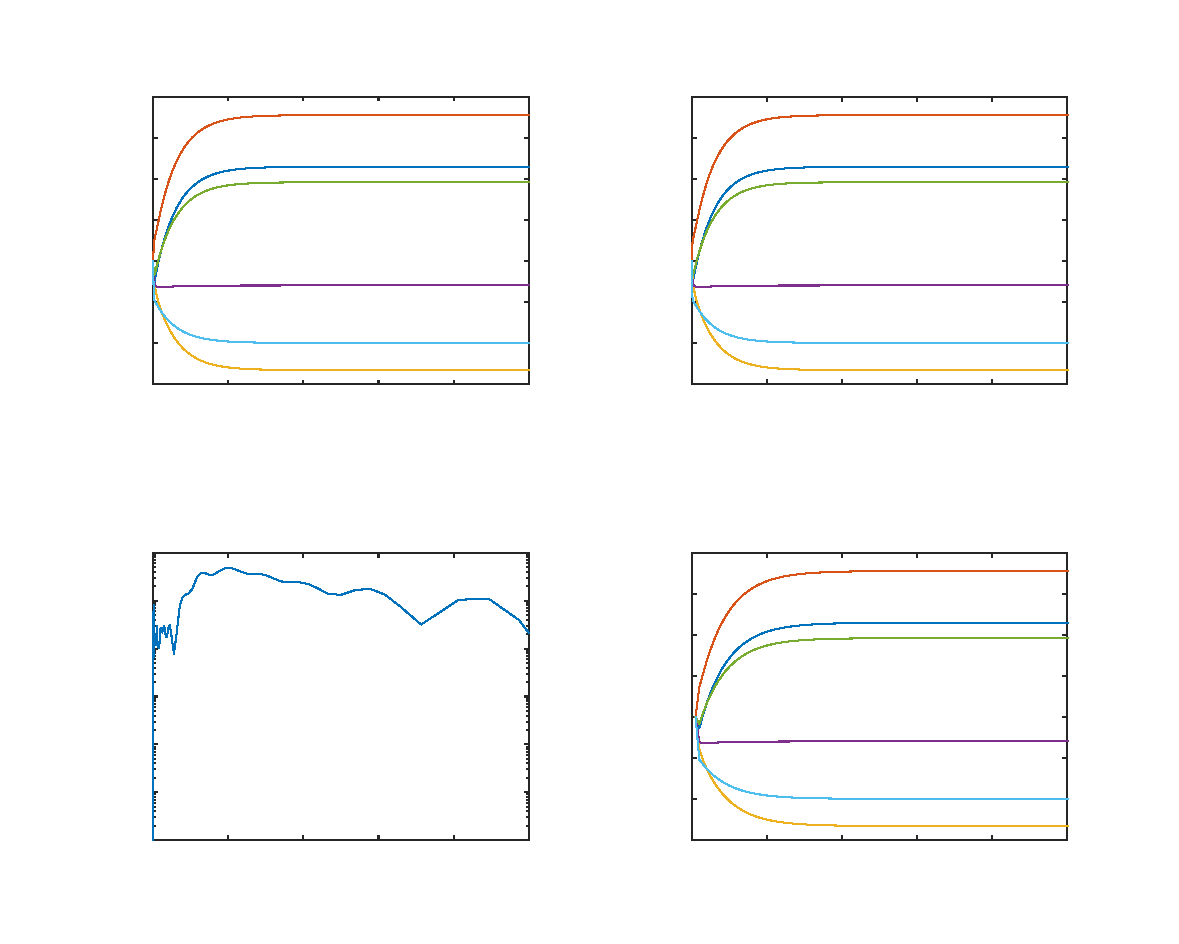
\includegraphics{Trajectory-inc}
\end{picture}%
\begin{picture}(566,453)(0,0)
\fontsize{10}{0}
\selectfont\put(73.5801,261.175){\makebox(0,0)[t]{\textcolor[rgb]{0.15,0.15,0.15}{{0}}}}
\fontsize{10}{0}
\selectfont\put(109.612,261.175){\makebox(0,0)[t]{\textcolor[rgb]{0.15,0.15,0.15}{{20}}}}
\fontsize{10}{0}
\selectfont\put(145.644,261.175){\makebox(0,0)[t]{\textcolor[rgb]{0.15,0.15,0.15}{{40}}}}
\fontsize{10}{0}
\selectfont\put(181.676,261.175){\makebox(0,0)[t]{\textcolor[rgb]{0.15,0.15,0.15}{{60}}}}
\fontsize{10}{0}
\selectfont\put(217.708,261.175){\makebox(0,0)[t]{\textcolor[rgb]{0.15,0.15,0.15}{{80}}}}
\fontsize{10}{0}
\selectfont\put(253.739,261.175){\makebox(0,0)[t]{\textcolor[rgb]{0.15,0.15,0.15}{{100}}}}
\fontsize{10}{0}
\selectfont\put(68.5757,268.672){\makebox(0,0)[r]{\textcolor[rgb]{0.15,0.15,0.15}{{-2}}}}
\fontsize{10}{0}
\selectfont\put(68.5757,288.379){\makebox(0,0)[r]{\textcolor[rgb]{0.15,0.15,0.15}{{-1}}}}
\fontsize{10}{0}
\selectfont\put(68.5757,308.086){\makebox(0,0)[r]{\textcolor[rgb]{0.15,0.15,0.15}{{0}}}}
\fontsize{10}{0}
\selectfont\put(68.5757,327.793){\makebox(0,0)[r]{\textcolor[rgb]{0.15,0.15,0.15}{{1}}}}
\fontsize{10}{0}
\selectfont\put(68.5757,347.5){\makebox(0,0)[r]{\textcolor[rgb]{0.15,0.15,0.15}{{2}}}}
\fontsize{10}{0}
\selectfont\put(68.5757,367.207){\makebox(0,0)[r]{\textcolor[rgb]{0.15,0.15,0.15}{{3}}}}
\fontsize{10}{0}
\selectfont\put(68.5757,386.913){\makebox(0,0)[r]{\textcolor[rgb]{0.15,0.15,0.15}{{4}}}}
\fontsize{10}{0}
\selectfont\put(68.5757,406.62){\makebox(0,0)[r]{\textcolor[rgb]{0.15,0.15,0.15}{{5}}}}
\fontsize{11}{0}
\selectfont\put(163.66,416.62){\makebox(0,0)[b]{\textcolor[rgb]{0,0,0}{{gsl solution in C}}}}
\fontsize{11}{0}
\selectfont\put(54.5757,337.646){\rotatebox{90}{\makebox(0,0)[b]{\textcolor[rgb]{0.15,0.15,0.15}{{x(t)}}}}}
\fontsize{11}{0}
\selectfont\put(163.66,248.175){\makebox(0,0)[t]{\textcolor[rgb]{0.15,0.15,0.15}{{t}}}}
\fontsize{10}{0}
\selectfont\put(332.071,261.175){\makebox(0,0)[t]{\textcolor[rgb]{0.15,0.15,0.15}{{0}}}}
\fontsize{10}{0}
\selectfont\put(368.103,261.175){\makebox(0,0)[t]{\textcolor[rgb]{0.15,0.15,0.15}{{20}}}}
\fontsize{10}{0}
\selectfont\put(404.134,261.175){\makebox(0,0)[t]{\textcolor[rgb]{0.15,0.15,0.15}{{40}}}}
\fontsize{10}{0}
\selectfont\put(440.166,261.175){\makebox(0,0)[t]{\textcolor[rgb]{0.15,0.15,0.15}{{60}}}}
\fontsize{10}{0}
\selectfont\put(476.198,261.175){\makebox(0,0)[t]{\textcolor[rgb]{0.15,0.15,0.15}{{80}}}}
\fontsize{10}{0}
\selectfont\put(512.23,261.175){\makebox(0,0)[t]{\textcolor[rgb]{0.15,0.15,0.15}{{100}}}}
\fontsize{10}{0}
\selectfont\put(327.066,268.672){\makebox(0,0)[r]{\textcolor[rgb]{0.15,0.15,0.15}{{-2}}}}
\fontsize{10}{0}
\selectfont\put(327.066,288.379){\makebox(0,0)[r]{\textcolor[rgb]{0.15,0.15,0.15}{{-1}}}}
\fontsize{10}{0}
\selectfont\put(327.066,308.086){\makebox(0,0)[r]{\textcolor[rgb]{0.15,0.15,0.15}{{0}}}}
\fontsize{10}{0}
\selectfont\put(327.066,327.793){\makebox(0,0)[r]{\textcolor[rgb]{0.15,0.15,0.15}{{1}}}}
\fontsize{10}{0}
\selectfont\put(327.066,347.5){\makebox(0,0)[r]{\textcolor[rgb]{0.15,0.15,0.15}{{2}}}}
\fontsize{10}{0}
\selectfont\put(327.066,367.207){\makebox(0,0)[r]{\textcolor[rgb]{0.15,0.15,0.15}{{3}}}}
\fontsize{10}{0}
\selectfont\put(327.066,386.913){\makebox(0,0)[r]{\textcolor[rgb]{0.15,0.15,0.15}{{4}}}}
\fontsize{10}{0}
\selectfont\put(327.066,406.62){\makebox(0,0)[r]{\textcolor[rgb]{0.15,0.15,0.15}{{5}}}}
\fontsize{11}{0}
\selectfont\put(422.15,416.62){\makebox(0,0)[b]{\textcolor[rgb]{0,0,0}{{analytical solution}}}}
\fontsize{11}{0}
\selectfont\put(313.066,337.646){\rotatebox{90}{\makebox(0,0)[b]{\textcolor[rgb]{0.15,0.15,0.15}{{$x(t)$}}}}}
\fontsize{11}{0}
\selectfont\put(422.15,248.175){\makebox(0,0)[t]{\textcolor[rgb]{0.15,0.15,0.15}{{$t$}}}}
\fontsize{10}{0}
\selectfont\put(73.5801,42.333){\makebox(0,0)[t]{\textcolor[rgb]{0.15,0.15,0.15}{{0}}}}
\fontsize{10}{0}
\selectfont\put(109.612,42.333){\makebox(0,0)[t]{\textcolor[rgb]{0.15,0.15,0.15}{{20}}}}
\fontsize{10}{0}
\selectfont\put(145.644,42.333){\makebox(0,0)[t]{\textcolor[rgb]{0.15,0.15,0.15}{{40}}}}
\fontsize{10}{0}
\selectfont\put(181.676,42.333){\makebox(0,0)[t]{\textcolor[rgb]{0.15,0.15,0.15}{{60}}}}
\fontsize{10}{0}
\selectfont\put(217.708,42.333){\makebox(0,0)[t]{\textcolor[rgb]{0.15,0.15,0.15}{{80}}}}
\fontsize{10}{0}
\selectfont\put(253.739,42.333){\makebox(0,0)[t]{\textcolor[rgb]{0.15,0.15,0.15}{{100}}}}
\fontsize{10}{0}
\selectfont\put(68.5757,49.8301){\makebox(0,0)[r]{\textcolor[rgb]{0.15,0.15,0.15}{{$10^{-9}$}}}}
\fontsize{10}{0}
\selectfont\put(68.5757,72.8213){\makebox(0,0)[r]{\textcolor[rgb]{0.15,0.15,0.15}{{$10^{-8}$}}}}
\fontsize{10}{0}
\selectfont\put(68.5757,95.8125){\makebox(0,0)[r]{\textcolor[rgb]{0.15,0.15,0.15}{{$10^{-7}$}}}}
\fontsize{10}{0}
\selectfont\put(68.5757,118.804){\makebox(0,0)[r]{\textcolor[rgb]{0.15,0.15,0.15}{{$10^{-6}$}}}}
\fontsize{10}{0}
\selectfont\put(68.5757,141.795){\makebox(0,0)[r]{\textcolor[rgb]{0.15,0.15,0.15}{{$10^{-5}$}}}}
\fontsize{10}{0}
\selectfont\put(68.5757,164.786){\makebox(0,0)[r]{\textcolor[rgb]{0.15,0.15,0.15}{{$10^{-4}$}}}}
\fontsize{10}{0}
\selectfont\put(68.5757,187.777){\makebox(0,0)[r]{\textcolor[rgb]{0.15,0.15,0.15}{{$10^{-3}$}}}}
\fontsize{11}{0}
\selectfont\put(163.66,197.777){\makebox(0,0)[b]{\textcolor[rgb]{0,0,0}{{Difference between gsl and analytical solution}}}}
\fontsize{11}{0}
\selectfont\put(22.5757,118.804){\rotatebox{90}{\makebox(0,0)[b]{\textcolor[rgb]{0.15,0.15,0.15}{{$\sum_i |x_i(t) - x_i(t;\texttt{gsl})|$}}}}}
\fontsize{11}{0}
\selectfont\put(163.66,29.333){\makebox(0,0)[t]{\textcolor[rgb]{0.15,0.15,0.15}{{$t$}}}}
\fontsize{10}{0}
\selectfont\put(332.071,42.333){\makebox(0,0)[t]{\textcolor[rgb]{0.15,0.15,0.15}{{0}}}}
\fontsize{10}{0}
\selectfont\put(368.103,42.333){\makebox(0,0)[t]{\textcolor[rgb]{0.15,0.15,0.15}{{20}}}}
\fontsize{10}{0}
\selectfont\put(404.134,42.333){\makebox(0,0)[t]{\textcolor[rgb]{0.15,0.15,0.15}{{40}}}}
\fontsize{10}{0}
\selectfont\put(440.166,42.333){\makebox(0,0)[t]{\textcolor[rgb]{0.15,0.15,0.15}{{60}}}}
\fontsize{10}{0}
\selectfont\put(476.198,42.333){\makebox(0,0)[t]{\textcolor[rgb]{0.15,0.15,0.15}{{80}}}}
\fontsize{10}{0}
\selectfont\put(512.23,42.333){\makebox(0,0)[t]{\textcolor[rgb]{0.15,0.15,0.15}{{100}}}}
\fontsize{10}{0}
\selectfont\put(327.066,49.8301){\makebox(0,0)[r]{\textcolor[rgb]{0.15,0.15,0.15}{{-2}}}}
\fontsize{10}{0}
\selectfont\put(327.066,69.5366){\makebox(0,0)[r]{\textcolor[rgb]{0.15,0.15,0.15}{{-1}}}}
\fontsize{10}{0}
\selectfont\put(327.066,89.2437){\makebox(0,0)[r]{\textcolor[rgb]{0.15,0.15,0.15}{{0}}}}
\fontsize{10}{0}
\selectfont\put(327.066,108.95){\makebox(0,0)[r]{\textcolor[rgb]{0.15,0.15,0.15}{{1}}}}
\fontsize{10}{0}
\selectfont\put(327.066,128.657){\makebox(0,0)[r]{\textcolor[rgb]{0.15,0.15,0.15}{{2}}}}
\fontsize{10}{0}
\selectfont\put(327.066,148.364){\makebox(0,0)[r]{\textcolor[rgb]{0.15,0.15,0.15}{{3}}}}
\fontsize{10}{0}
\selectfont\put(327.066,168.071){\makebox(0,0)[r]{\textcolor[rgb]{0.15,0.15,0.15}{{4}}}}
\fontsize{10}{0}
\selectfont\put(327.066,187.777){\makebox(0,0)[r]{\textcolor[rgb]{0.15,0.15,0.15}{{5}}}}
\fontsize{11}{0}
\selectfont\put(422.15,197.777){\makebox(0,0)[b]{\textcolor[rgb]{0,0,0}{{lsode solution in \emph{GNU Octave}}}}}
\fontsize{11}{0}
\selectfont\put(313.066,118.804){\rotatebox{90}{\makebox(0,0)[b]{\textcolor[rgb]{0.15,0.15,0.15}{{$x(t)$}}}}}
\fontsize{11}{0}
\selectfont\put(422.15,29.333){\makebox(0,0)[t]{\textcolor[rgb]{0.15,0.15,0.15}{{$t$}}}}
\end{picture}

  \caption[trajectory accuracy of gsl solvers]{Accuracy of the
    trajectory $x(t_j)$ using the gsl solvers in
    \texttt{gsl\_odeiv2.h} as compared to the analytical
    solution~\eqref{eq:sol}. For completeness, we also include the
    numerical solution from \emph{GNU Octave}'s \texttt{lsode} solver
    for stiff problems. Bottom left: the absolute difference between
    the trajectories, summed over all state variables.}
\label{fig:trajectory}
\end{figure}

\begin{figure}
  \centering\sffamily\firalining
  \hspace*{-2cm}% Title: gl2ps_renderer figure
% Creator: GL2PS 1.4.0, (C) 1999-2017 C. Geuzaine
% For: Octave
% CreationDate: Thu Apr 29 22:37:36 2021
\setlength{\unitlength}{1pt}
\begin{picture}(0,0)
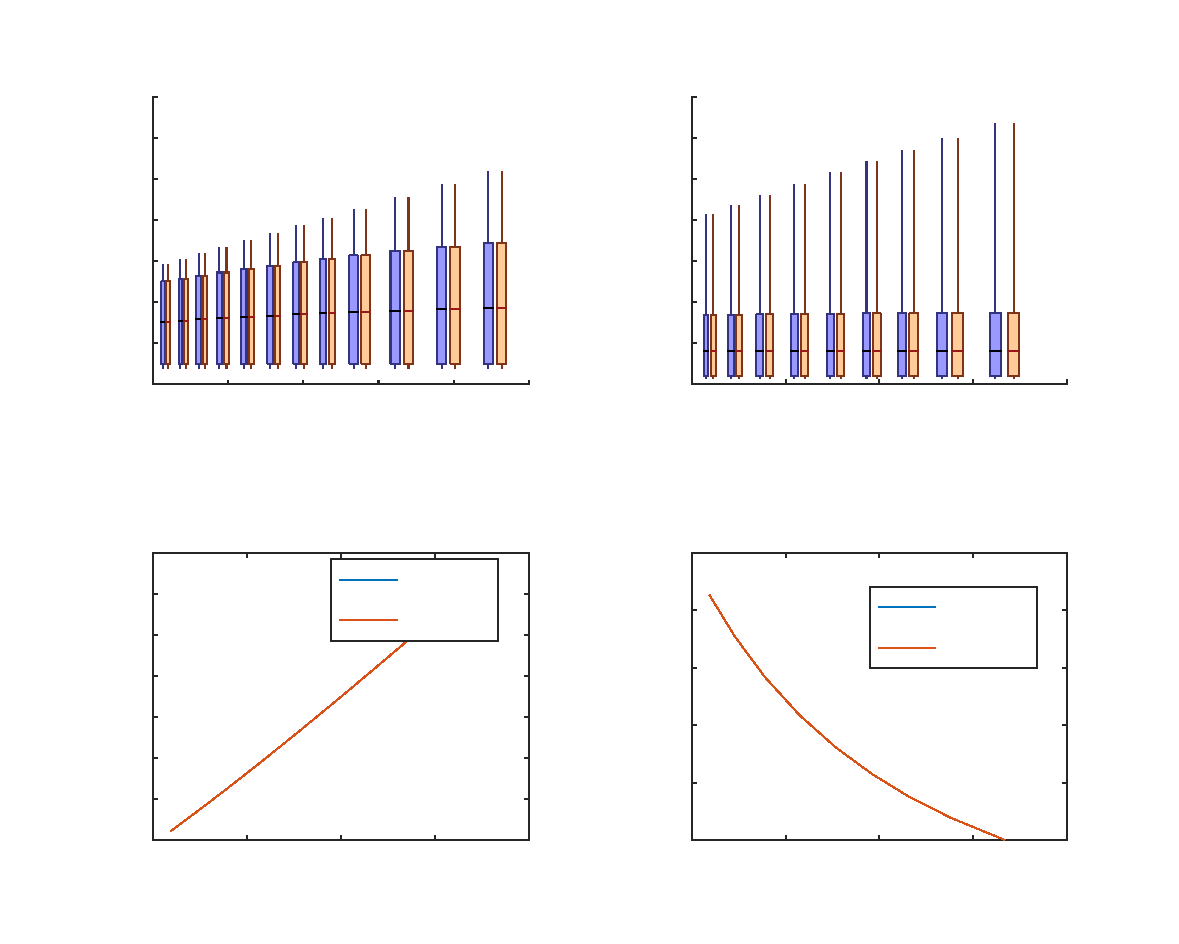
\includegraphics{FisherInformation-inc}
\end{picture}%
\begin{picture}(566,453)(0,0)
\fontsize{10}{0}
\selectfont\put(73.5801,261.175){\makebox(0,0)[t]{\textcolor[rgb]{0.15,0.15,0.15}{{0.5}}}}
\fontsize{10}{0}
\selectfont\put(109.612,261.175){\makebox(0,0)[t]{\textcolor[rgb]{0.15,0.15,0.15}{{0.6}}}}
\fontsize{10}{0}
\selectfont\put(145.644,261.175){\makebox(0,0)[t]{\textcolor[rgb]{0.15,0.15,0.15}{{0.7}}}}
\fontsize{10}{0}
\selectfont\put(181.676,261.175){\makebox(0,0)[t]{\textcolor[rgb]{0.15,0.15,0.15}{{0.8}}}}
\fontsize{10}{0}
\selectfont\put(217.708,261.175){\makebox(0,0)[t]{\textcolor[rgb]{0.15,0.15,0.15}{{0.9}}}}
\fontsize{10}{0}
\selectfont\put(253.739,261.175){\makebox(0,0)[t]{\textcolor[rgb]{0.15,0.15,0.15}{{1}}}}
\fontsize{10}{0}
\selectfont\put(68.5757,268.672){\makebox(0,0)[r]{\textcolor[rgb]{0.15,0.15,0.15}{{0}}}}
\fontsize{10}{0}
\selectfont\put(68.5757,288.379){\makebox(0,0)[r]{\textcolor[rgb]{0.15,0.15,0.15}{{0.2}}}}
\fontsize{10}{0}
\selectfont\put(68.5757,308.086){\makebox(0,0)[r]{\textcolor[rgb]{0.15,0.15,0.15}{{0.4}}}}
\fontsize{10}{0}
\selectfont\put(68.5757,327.793){\makebox(0,0)[r]{\textcolor[rgb]{0.15,0.15,0.15}{{0.6}}}}
\fontsize{10}{0}
\selectfont\put(68.5757,347.5){\makebox(0,0)[r]{\textcolor[rgb]{0.15,0.15,0.15}{{0.8}}}}
\fontsize{10}{0}
\selectfont\put(68.5757,367.207){\makebox(0,0)[r]{\textcolor[rgb]{0.15,0.15,0.15}{{1}}}}
\fontsize{10}{0}
\selectfont\put(68.5757,386.913){\makebox(0,0)[r]{\textcolor[rgb]{0.15,0.15,0.15}{{1.2}}}}
\fontsize{10}{0}
\selectfont\put(68.5757,406.62){\makebox(0,0)[r]{\textcolor[rgb]{0.15,0.15,0.15}{{1.4}}}}
\fontsize{11}{0}
\selectfont\put(163.66,247.175){\makebox(0,0)[t]{\textcolor[rgb]{0.15,0.15,0.15}{{$t$}}}}
\fontsize{11}{0}
\selectfont\put(49.5757,337.646){\rotatebox{90}{\makebox(0,0)[b]{\textcolor[rgb]{0.15,0.15,0.15}{{singular values of $S(t)$ \texttt{svd}}}}}}
\fontsize{11}{0}
\selectfont\put(163.66,416.62){\makebox(0,0)[b]{\textcolor[rgb]{0,0,0}{{gsl odeiv2 solution (blue) analytical (orange)}}}}
\fontsize{10}{0}
\selectfont\put(332.071,261.175){\makebox(0,0)[t]{\textcolor[rgb]{0.15,0.15,0.15}{{2}}}}
\fontsize{10}{0}
\selectfont\put(377.11,261.175){\makebox(0,0)[t]{\textcolor[rgb]{0.15,0.15,0.15}{{2.5}}}}
\fontsize{10}{0}
\selectfont\put(422.15,261.175){\makebox(0,0)[t]{\textcolor[rgb]{0.15,0.15,0.15}{{3}}}}
\fontsize{10}{0}
\selectfont\put(467.19,261.175){\makebox(0,0)[t]{\textcolor[rgb]{0.15,0.15,0.15}{{3.5}}}}
\fontsize{10}{0}
\selectfont\put(512.23,261.175){\makebox(0,0)[t]{\textcolor[rgb]{0.15,0.15,0.15}{{4}}}}
\fontsize{10}{0}
\selectfont\put(327.066,268.672){\makebox(0,0)[r]{\textcolor[rgb]{0.15,0.15,0.15}{{0}}}}
\fontsize{10}{0}
\selectfont\put(327.066,288.379){\makebox(0,0)[r]{\textcolor[rgb]{0.15,0.15,0.15}{{0.5}}}}
\fontsize{10}{0}
\selectfont\put(327.066,308.086){\makebox(0,0)[r]{\textcolor[rgb]{0.15,0.15,0.15}{{1}}}}
\fontsize{10}{0}
\selectfont\put(327.066,327.793){\makebox(0,0)[r]{\textcolor[rgb]{0.15,0.15,0.15}{{1.5}}}}
\fontsize{10}{0}
\selectfont\put(327.066,347.5){\makebox(0,0)[r]{\textcolor[rgb]{0.15,0.15,0.15}{{2}}}}
\fontsize{10}{0}
\selectfont\put(327.066,367.207){\makebox(0,0)[r]{\textcolor[rgb]{0.15,0.15,0.15}{{2.5}}}}
\fontsize{10}{0}
\selectfont\put(327.066,386.913){\makebox(0,0)[r]{\textcolor[rgb]{0.15,0.15,0.15}{{3}}}}
\fontsize{10}{0}
\selectfont\put(327.066,406.62){\makebox(0,0)[r]{\textcolor[rgb]{0.15,0.15,0.15}{{3.5}}}}
\fontsize{11}{0}
\selectfont\put(422.15,248.175){\makebox(0,0)[t]{\textcolor[rgb]{0.15,0.15,0.15}{{$t$}}}}
\fontsize{11}{0}
\selectfont\put(309.066,337.646){\rotatebox{90}{\makebox(0,0)[b]{\textcolor[rgb]{0.15,0.15,0.15}{{singular values of $S(t)$ \texttt{svd}}}}}}
\fontsize{11}{0}
\selectfont\put(422.15,416.62){\makebox(0,0)[b]{\textcolor[rgb]{0,0,0}{{gsl odeiv2 solution (blue) analytical (orange)}}}}
\fontsize{10}{0}
\selectfont\put(73.5801,42.333){\makebox(0,0)[t]{\textcolor[rgb]{0.15,0.15,0.15}{{2}}}}
\fontsize{10}{0}
\selectfont\put(118.62,42.333){\makebox(0,0)[t]{\textcolor[rgb]{0.15,0.15,0.15}{{2.5}}}}
\fontsize{10}{0}
\selectfont\put(163.66,42.333){\makebox(0,0)[t]{\textcolor[rgb]{0.15,0.15,0.15}{{3}}}}
\fontsize{10}{0}
\selectfont\put(208.7,42.333){\makebox(0,0)[t]{\textcolor[rgb]{0.15,0.15,0.15}{{3.5}}}}
\fontsize{10}{0}
\selectfont\put(253.739,42.333){\makebox(0,0)[t]{\textcolor[rgb]{0.15,0.15,0.15}{{4}}}}
\fontsize{10}{0}
\selectfont\put(68.5757,49.8301){\makebox(0,0)[r]{\textcolor[rgb]{0.15,0.15,0.15}{{4}}}}
\fontsize{10}{0}
\selectfont\put(68.5757,69.5366){\makebox(0,0)[r]{\textcolor[rgb]{0.15,0.15,0.15}{{5}}}}
\fontsize{10}{0}
\selectfont\put(68.5757,89.2437){\makebox(0,0)[r]{\textcolor[rgb]{0.15,0.15,0.15}{{6}}}}
\fontsize{10}{0}
\selectfont\put(68.5757,108.95){\makebox(0,0)[r]{\textcolor[rgb]{0.15,0.15,0.15}{{7}}}}
\fontsize{10}{0}
\selectfont\put(68.5757,128.657){\makebox(0,0)[r]{\textcolor[rgb]{0.15,0.15,0.15}{{8}}}}
\fontsize{10}{0}
\selectfont\put(68.5757,148.364){\makebox(0,0)[r]{\textcolor[rgb]{0.15,0.15,0.15}{{9}}}}
\fontsize{10}{0}
\selectfont\put(68.5757,168.071){\makebox(0,0)[r]{\textcolor[rgb]{0.15,0.15,0.15}{{10}}}}
\fontsize{10}{0}
\selectfont\put(68.5757,187.777){\makebox(0,0)[r]{\textcolor[rgb]{0.15,0.15,0.15}{{11}}}}
\fontsize{11}{0}
\selectfont\put(163.66,197.777){\makebox(0,0)[b]{\textcolor[rgb]{0,0,0}{{Fisher Information (norm)}}}}
\fontsize{11}{0}
\selectfont\put(53.5757,118.804){\rotatebox{90}{\makebox(0,0)[b]{\textcolor[rgb]{0.15,0.15,0.15}{{$\|\texttt{FI}(t)\|$}}}}}
\fontsize{11}{0}
\selectfont\put(163.66,29.333){\makebox(0,0)[t]{\textcolor[rgb]{0.15,0.15,0.15}{{$t$}}}}
\fontsize{9}{0}
\selectfont\put(194.598,174.925){\makebox(0,0)[l]{\textcolor[rgb]{0,0,0}{{analytical}}}}
\fontsize{9}{0}
\selectfont\put(194.598,155.331){\makebox(0,0)[l]{\textcolor[rgb]{0,0,0}{{gsl}}}}
\fontsize{10}{0}
\selectfont\put(332.071,42.333){\makebox(0,0)[t]{\textcolor[rgb]{0.15,0.15,0.15}{{2}}}}
\fontsize{10}{0}
\selectfont\put(377.11,42.333){\makebox(0,0)[t]{\textcolor[rgb]{0.15,0.15,0.15}{{2.5}}}}
\fontsize{10}{0}
\selectfont\put(422.15,42.333){\makebox(0,0)[t]{\textcolor[rgb]{0.15,0.15,0.15}{{3}}}}
\fontsize{10}{0}
\selectfont\put(467.19,42.333){\makebox(0,0)[t]{\textcolor[rgb]{0.15,0.15,0.15}{{3.5}}}}
\fontsize{10}{0}
\selectfont\put(512.23,42.333){\makebox(0,0)[t]{\textcolor[rgb]{0.15,0.15,0.15}{{4}}}}
\fontsize{10}{0}
\selectfont\put(327.066,49.8301){\makebox(0,0)[r]{\textcolor[rgb]{0.15,0.15,0.15}{{0.3}}}}
\fontsize{10}{0}
\selectfont\put(327.066,77.4194){\makebox(0,0)[r]{\textcolor[rgb]{0.15,0.15,0.15}{{0.4}}}}
\fontsize{10}{0}
\selectfont\put(327.066,105.009){\makebox(0,0)[r]{\textcolor[rgb]{0.15,0.15,0.15}{{0.5}}}}
\fontsize{10}{0}
\selectfont\put(327.066,132.599){\makebox(0,0)[r]{\textcolor[rgb]{0.15,0.15,0.15}{{0.6}}}}
\fontsize{10}{0}
\selectfont\put(327.066,160.188){\makebox(0,0)[r]{\textcolor[rgb]{0.15,0.15,0.15}{{0.7}}}}
\fontsize{10}{0}
\selectfont\put(327.066,187.777){\makebox(0,0)[r]{\textcolor[rgb]{0.15,0.15,0.15}{{0.8}}}}
\fontsize{11}{0}
\selectfont\put(422.15,197.777){\makebox(0,0)[b]{\textcolor[rgb]{0,0,0}{{Fisher Information (reciprocal condition number)}}}}
\fontsize{11}{0}
\selectfont\put(308.066,118.804){\rotatebox{90}{\makebox(0,0)[b]{\textcolor[rgb]{0.15,0.15,0.15}{{$\text{rcond}(\texttt{FI}) / 10^{-3}$}}}}}
\fontsize{11}{0}
\selectfont\put(422.15,29.333){\makebox(0,0)[t]{\textcolor[rgb]{0.15,0.15,0.15}{{$t$}}}}
\fontsize{9}{0}
\selectfont\put(453.088,161.713){\makebox(0,0)[l]{\textcolor[rgb]{0,0,0}{{analytical}}}}
\fontsize{9}{0}
\selectfont\put(453.088,142.119){\makebox(0,0)[l]{\textcolor[rgb]{0,0,0}{{gsl}}}}
\end{picture}

  \caption[Sensitivity Approximation]{The accuracy of the sensitivity
    matrix is summarized as a box-and-whisker plot of the singular
    values of $S(x,t;p)$ (singular value decomposition, per time
    point), this is to reduce visual clutter, not to imply that the
    values are random. In (blue) the approximated sensitivity, in
    (orange) the analytical solution. The numerical approximation
    eventually diverges, when the system approaches steady
    state. Lower panels show the accuracy of the Fisher information:
    $\texttt{FI} = S^{\text{T}}S$ (this is assuming a Gaussian error
    model with unit noise parameter and corresponding Likelihood
    function).}
\label{fig:fi}
\end{figure}

\end{document}